\documentclass[a4paper,12pt]{article}

\usepackage[in]{fullpage}
\usepackage{parskip}
\usepackage{tikz}
\usepackage[backend=bibtex,style=numeric-comp,sorting=none,sortcites=true]{biblatex}

\title{Qualifying Dissertation}
\author{James Baxter}
\date{}

\bibliography{literature} 

\begin{document}
\maketitle

\section{Introduction}
\begin{itemize}
  \item Popularity of Java
  \item Use of Java in embedded systems
  \item Importance of program correctness
  \item Importance of compiler correctness
  \item Difficulties of Java on embedded systems
  \item The need for a correct SCJ compiler for embedded systems
\end{itemize}

\section{Literature Review}

As the correctness of the compiler is of great importance to the correctness of the programs produced using it, there has been much research in the past into compiler correctness.
The approach that was used in the earliest works on compiler correctness, which is still widely used today, is to show that a diagram of the form shown in Figure~\ref{commuting-diagram} commutes.
\begin{figure}
  \begin{center}
    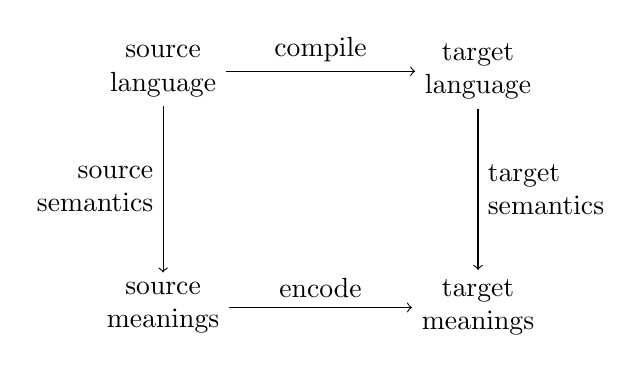
\begin{tikzpicture}
      \node[align=center] (S) at (0cm,3cm) {source\\language};
      \node[align=center] (T) at (4cm,3cm) {target\\language};
      \node[align=center] (M) at (0cm,0cm) {source\\meanings};
      \node[align=center] (U) at (4cm,0cm) {target\\meanings};
      
      \path (S) edge[->] node[align=center, above] {compile}           (T);
      \path (S) edge[->] node[align=right, left]   {source\\semantics} (M);
      \path (T) edge[->] node[align=left, right]   {target\\semantics} (U);
      \path (M) edge[->] node[align=center, above] {encode}            (U);
    \end{tikzpicture}
  \end{center}
  \caption{The commuting diagram used in the traditional approach to compiler verification}
  \label{commuting-diagram}
\end{figure}
Lockwood Morris\cite{morris1973} first observed that the commuting diagram approach was the usual approach to showing compiler correctness, though his version of the diagram had a decode function relating target meanings to source meanings.
Thatcher \emph{et al.}\cite{thatcher1979}, in extending Lockwood Morris' verification of a compiler, noticed that an encode function was more useful in reasoning and so included it in their diagram instead of the decode function.

The commuting diagram approach can be seen in some of the earliest work on compiler correctness, particularly McCarthy and Painter's paper from 1967\cite{mccarthy1967}.
McCarthy and Painter show the correctness of a compiler for a very simple expression language that targets a simple 4-instruction machine.
The source language consists only of constants, variables and addition to form expressions such as $(x + 3) + (y + z)$, and a function that evaluates these expressions to values under a particular variable binding forns the semantics of the source language.
The target machine consists of an acumulator register and a memory store with four instructions:
\begin{itemize}
  \item LI $\alpha$ --- which loads the immediate value $\alpha$ into the accumulator
  \item LOAD $x$ --- which loads a value from the memory location $x$ into the accumulator
  \item STO $x$ --- which stores the value in the accumulator in memory location $x$
  \item ADD $x$ --- which add the value at memory location $x$ to the value in the accumulator
\end{itemize}
The semantics of this target machine are defined by a function that takes an intial state and a list of instructions and outputs the final state.
McCarthy and Painter then define a compilation function from the source language to the target language.
The correctness of the compiler is defined by providing a function that puts the computed value of an expression into the accumulator of a machine state. 
It is then required that applying the function to the result of evaluating an expression is equivalent under a partial equality relation to the resultant state from compiling and running the expression.
The reason for the use of a partial equality is to ensure that any temporary variables introduced in compilation are ignored when comparing the machine states.
Though the use of partial equality and the equational way in which McCarthy and Painter state their definition of compiler correctness obscures it slightly, this can be seen as following the commuting diagram approach as shown in Figure~\ref{mccarthy1967-diagram}.
\begin{figure}
  \begin{center}
    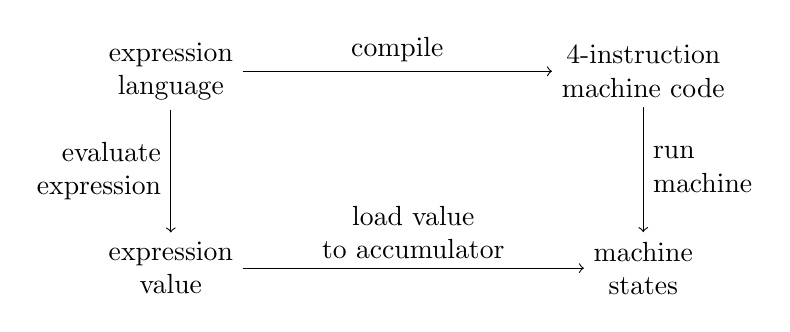
\begin{tikzpicture}
      \node[align=center] (S) at (0cm,2.5cm) {expression\\language};
      \node[align=center] (T) at (6cm,2.5cm) {4-instruction\\machine code};
      \node[align=center] (M) at (0cm,0cm)   {expression\\value};
      \node[align=center] (U) at (6cm,0cm)   {machine\\states};
      
      \path (S) edge[->] node[align=center, above] {compile}                    (T);
      \path (S) edge[->] node[align=right, left]   {evaluate\\expression}       (M);
      \path (T) edge[->] node[align=left, right]   {run\\machine}               (U);
      \path (M) edge[->] node[align=center, above] {load value\\to accumulator} (U);
    \end{tikzpicture}
  \end{center}
  \caption{A diagram showing how McCarthy and Painter's definition of compiler correctness follows the commuting diagram approach}
  \label{mccarthy1967-diagram}
\end{figure}
\end{document}